% !TEX encoding = UTF-8 Unicode
% !TEX spellcheck = en_US

\documentclass[runningheads]{llncs}
%
%%% packages
\usepackage{paralist}
\usepackage{amsmath}
\usepackage{amssymb}
\usepackage{siunitx}
\usepackage{graphicx}\graphicspath{{./figures/}}
\usepackage[T1]{fontenc} % Für Unterstrich in URL
\usepackage[utf8]{inputenc} % Für Deutsche Umlaute
\usepackage{orcidlink}
% to typeset URLs, URIs, and DOIs
\usepackage{url}
\def\UrlFont{\rmfamily}
\usepackage{subfigure}
\usepackage{todonotes}
\usepackage{wrapfig}

%%%% commands
\newcommand{\imgscaled}[4]{
	\begin{figure}[#3]
	\centering
	\vspace{-5mm}
    \includegraphics[width=#4\textwidth]{#1}
    \caption{#2} \label{fig:#1}
    \vspace{-5mm}
    \end{figure}}
\newcommand{\pdftexscaled}[4]{
	\begin{figure}[#3]
	\centering
	\vspace{-5mm}
	\def\svgwidth{#4\columnwidth}
    \input{#1}
    \caption{#2} \label{fig:#1}
    \vspace{-5mm}
    \end{figure}}
\newcommand{\TODO}[1]{\textcolor{red}{\textbf{TODO: #1}}}
% Mathematik
\renewcommand{\vec}[1]{\mbox{\boldmath{$#1$}}}
\newcommand{\transpose}{{\mathrm{T}}}
\newcommand{\ind}[1]{{\mathrm{#1}}}
\newcommand{\cf}[1]{\ind{(CF)}_\ind{#1}}
\newcommand{\tmat}[2]{{^{\mathrm{#1}}\vec{T}_{\mathrm{#2}}}}
\newcommand{\rmat}[2]{{^{\mathrm{#1}}\vec{R}_{\mathrm{#2}}}}
\newcommand{\invmat}[1]{  \left( #1 \right)^{-1}  }
\graphicspath{{./figures/}}
% If you use the hyperref package, please uncomment the following line
% to display URLs in blue roman font according to Springer's eBook style:
% \renewcommand\UrlFont{\color{blue}\rmfamily}
\begin{document}
%
% \title{Contribution Title}
% ----- Titelvarianten
%\title{Task-Adapted Synthesis and Design of a 6-DoF Parallel Robot for Weed Control}
% \title{Combined Structural and Dimensional Synthesis and Design of a 6-DoF Parallel Robot\\ for Weed Control}
\title{Task-Specific Synthesis and Design of a mobile six-DoF Hexa Parallel Robot for Weed Control}
% keywords:
% synthesis, parallel robot, 6DoF, weed control
%------

\titlerunning{Synthesis and Design of a six-DoF Parallel Robot for Weed Control}
% If the paper title is too long for the running head, you can set
% an abbreviated paper title here
%

% \author{Tim Sterneck\inst{1}\orcidID{0000-0003-1649-9371} \and 
% Jannik Fettin\inst{1}\orcidID{0000-0002-3544-2437} \and
% Moritz Schappler\inst{1}\orcidID{0000-0001-7952-7363} }

\author{Tim Sterneck\inst{1}\orcidlink{0000-0003-1649-9371} \and 
Jannik Fettin\inst{1}\orcidlink{0000-0002-3544-2437} \and
Moritz Schappler\inst{1}\orcidlink{0000-0001-7952-7363} }
%
\authorrunning{T. Sterneck et al.}
% First names are abbreviated in the running head.
% If there are more than two authors, 'et al.' is used.
%
\institute{Institute of Mechatronic Systems, Leibniz University of Hannover, Germany\\
\email{\{firstname.lastname\}@imes.uni-hannover.de}}
%
\maketitle              % typeset the header of the contribution
%
\begin{abstract}
In automated weed control, kinematics of varying complexity are required for tool guidance, depending on the weeding principle. 
Mechanical tools in particular require several degrees of freedom (DoF) in order to operate in a plant-specific way, which can be realized by parallel kinematic machines due to their dynamic performance. 
The development of a kinematic structure under task-specific requirements is done using combined structural and dimensional synthesis and a detailed manual design stage, which leads to a new variant of the six-DoF \textsc{Hexa} robot. %, which turns out to be beneficial in the present scenario. 
\keywords{SDG6 \and SDG11 \and SDG12 \and Hexa parallel robot \and weed control}
\end{abstract}
%
%%%%%%%%%%%%%%
\section{Introduction and State of the Art}
%Introduction with reference to: \\
%Sustainable Goals:\\
%- SDG6 (Clean Water and Sanitation): avoidance of herbicides and pollution %of (ground) water\\
%- SDG11 (sustainable cities and communities): sustainable agriculture as %element in sustainable communities\\
%- SDG12 (responsible consumption and production): food has big part in the %consumption and production of civilizations \\
%\\
\begin{wrapfigure}{r}{0.3\textwidth}
    \centering
	\vspace{-8mm}
	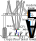
\includegraphics[width=1.0\linewidth]{weeding_system.pdf}
	\caption{Scheme of the presented weeding system}
	\label{fig:application_scenario}
	\vspace{-7mm}
\end{wrapfigure}
For most crops in agriculture weed control effort is required due to the competition for biological resources. 
Still the most widely used approach is applying herbicides, which are economical but come with downsides, as they are usually non-selective and partly inefficient. 
Herbicides and their degradation products can even infiltrate unintended areas as water bodies, which should be avoided with respect to negative effects on human and animal health. 
Using automated robotic systems is a promising alternative since manual weeding is expensive. 
In this paper, we are focusing on the kinematic aspect of robotics for tool handling rather than on the topic of mobile robots e.g. carrying the weeding tools, as shown in Fig~\ref{fig:application_scenario}. 
In the following, we refer to this as parallel kinematic machine (PKM).

% 
%%%% Notizen
% - need for weed control due to economic efficiency\\
% - high importance especially in the early growth stage\\
% - currently the preferred approach for weed control is still the usage of herbicides\\
% - sales volume remains at a high level in recent years\\
% % Absatz DE: https://de.statista.com/statistik/daten/studie/154717/umfrage/entwicklung-des-absatzes-von-herbiziden-in-deutschland/
% %
% - cheap, easy and fast application\\
% - downsides: \\
%     * non selective usage, mostly overdosage -> low efficiency\\
%     * unclear/controversial effects (of herbicides and herbicide degradation products) on human and animal health\\
%     * infiltration into water bodies and groundwater\\
%     * processes involved in the movement of pesticides: Metabolism in the crop, wind erosion of treated soil, vapour drift, chemical and microbial degradation in water/soil, rainfall washout, leaching and preferential flow \cite{Martin2016}\\
% - avoidance of herbicides preserves health of water bodies and eliminates remaining human health risk\\
%- mechanical weed removal, which is necessary at the advanced stage of growth is possible through expensive manual work\\
% - using automated robotic systems is promising also in terms of cost to compete with the use of herbicides.\\
% - here we are focusing on robotics in sense of kinematics for moving tools, not on the topic of mobile robotics\\
% - focusing on parallel robotics, due to pick-and-place-like task\\
% - Since not all mechanical methods for weed removal are 3T0R tasks and can be solved with common kinematics (such as the Delta robot), a crucial part of the development is synthesis in the sense of finding the best structure and kinematic parameters\\
% - requires 3T2R task\\
%     * accessibility of the plant roots\\
%

% \subsection*{Related Works}     % Abschnitt nur zur Strukturierung der Notizen
Weeding robots can be categorized according to the operating principle of the weeding tool (mechanical, chemical, electric discharge, laser irradiation, water jet treatment), and accordingly different requirements exist for tool handling.%manipulating the tool. 

%%%% Systeme ohne aktive Werkzeugpositionierung
In numerous applications, the movement of the carrier system is used, so no further kinematics is required for tool positioning. 
The ``Ecorobotix ARA'' \cite{Ecorobotix} uses a large array of individually controllable nozzles to fine-dose herbicides, a similar principle is applied in \cite{Utstumo2018}. 
There are also systems for weed removal by laser irradiation, as in the ``Carbon Robotics LaserWeeder'' \cite{CarbonRobotics}, which works without an additional tool positioning. 
\cite{Zhang2022} shows more examples of mechanical weeding, both with rotating tools, and completely passive. 
% - Ecorobotix \cite{Ecorobotix}\\
%     * chemical processing\\
%     * no tool handling kinematic, row of individually controllable nozzles\\
%     * delta kinematics used in an earlier version\\
% - Carbon Robotics LaserWeeder \cite{CarbonRobotics}\\
%     * laser modules\\
%     * no tool handling kinematic\\
% % Quellen auch im Review Zhang
% - Tertill robotic weeder \cite{Sanchez2021}
%     * desingned for home gardeners\\
%     * mechanical weed whacker tool\\
%     * no tool handling kinematic,  positioning by mobile robot itself\\
% - \cite{Sori2018}\\
%     * mechanical rot. tool\\
%     * no tool handling kinematic\\
% - \cite{Uchida2019}\\
%     * mechanical, passiv\\
%     * no tool handling\\
% - \cite{Utstumo2018}\\
%     * spray system\\
%     * nozzle array, no tool handling kinematic\\
    
%%%% Systeme mit 1-2dof Werkzeugpositionierung
Selective weeding using mechanical tools requires at least one degree of freedom (DoF) for tool positioning. 
``Bonirob'', a multifunctional mobile agriculture robot introduced in \cite{Ruckelshausen2009} was used for weeding with fixed nozzles and additional linear actuated stamps. 
Other systems with one-DoF tool positioning include the ``Naio Technologies OZ'' \cite{NaioTechnologies} with various tools, the ``Carre Aggriculture Anatis'' \cite{CarbonRobotics} and the ``Farmdroid'' \cite{Farmdroid}, both with one-DoF digging tools. 
In the Farming Revolution ``Farming GT'' \cite{farming_revolution} the rotating tool is guided by two-DoF serial kinematics. 
Further applications with mechanical tools, lasers or water jets can be found in \cite{Zhang2022}, containing only serial kinematics. 
% - Bonirob, introduced in \cite{Ruckelshausen2009}\\
%     * multifunctional mobile robot\\
%     * spraying tools and lin. stamp were used (1 dof linear tool handling)\\
% - oz (naio technologies) \cite{NaioTechnologies}\\
%     * mechanical weeding, multiple tools\\
%     * 1 dof tool handling (vertical)\\
% - Farming GT (Farming revolution) \cite{farming_revolution}\\
%     * mechanincal, rot. tool\\
%     * 2 dof serial tool handling kinematics\\
% - Anatis (Carre agriculture) \cite{CARRE}\\
%     * mechanical weeding\\
%     * 1 dof tool handling (vertical)\\
% - FarmDroid \cite{Farmdroid}\\
%     * mechanical weeding\\
%     * 1 dof tool handling (horizontal)\\
% % Quellen auch im Review Zhang
% - \cite{Bawden2017}\\
%     * mechanical and water spray system combined\\
%     * 1 and 2 DoF serial, linear kinematics\\
% - \cite{Xiong2017}\\
%     * laser\\
%     * 2dof serial gimbal kinematics\\


%%% Systeme mit >2dof Werkzeugpositionierung
Systems with tool handling kinematics of three or more DoF can be used for single-plant-based application. 
Providing high dynamics and a proven design, Delta robots are used in several weeding systems for tool handling, e.g. in the prototype of ``Small Robot Company'' \cite{SmallRobotCompany24-01-2023} with a linear Delta and an electrode, and by Ecorobotix \cite{Ecorobotix} with Delta robots for positioning nozzles in an earlier version. 
Serial kinematics, as in the SwagBot \cite{Eiffert2021}, where a six-DoF robotic arm positions a nozzle, are barely represented and not promising for an efficient application. 
In \cite{Blasco2002} a six-DoF parallel robot, the \textsc{Hexa} introduced in \cite{Pierrot1991}, was used, but primarily for positioning the camera system rather than the weeding tool. 
% - Small robot company \cite{SmallRobotCompany24.01.2023}\\
%     * prototype, electrical weeding\\
%     * 3 dof tool handling, linear delta robot\\
% - Ecorobotix\\
%     * chemical processing\\
%     * delta kinematics used in an earlier version\\
% - \cite{Blasco2002}\\
%     * electrical weeding\\
%     * 6dof hexa kinematics\\
Further applications for all types of tool handling can be found in the reviews~\cite{Zhang2022,Fountas2020,Oliveira2021}. 

Unlike the references above, we pursue the idea of a six-DoF parallel robot which is able to provide \emph{spatial orientation} of the \emph{rotating tool} prototype to be tested, which opens more possibilities for weed control.
This is similar to industrial machining tasks, where the task DoF can be termed as 3T2R, i.e. three translations and two rotations are defined.
% Since not all mechanical methods for weed control can be handled by existing robot designs, 
The crucial part of the development of such a weeding robot is the kinematic synthesis. % in the sense of finding the best structure and kinematic parameters. 
\emph{Combined structural and dimensional synthesis} is a suitable method for this purpose especially for parallel robots, introduced in \cite{Krefft2006} also at the example of a \textsc{Hexa} robot. 
% However, this procedure is not described for the development of robots for handling weeding tools yet. 
% Since the desired spatial orientation of our rotating tool presents a 3T2R task, 
Using this method, we present the development of parallel robot  with the following \emph{contributions}:
% Hexa-Literatur\\
% - \cite{Krefft2006}: Optimierung vom BS-Hexa\\
% - ggf. BS-Gruppe\\
% - combined structural and dimensional synthesis for PKM, introduced by \cite{Krefft2006}\todo{knapp!}\\
% * bisher nicht in Literatur zu weeding robots zu finden \\
% \subsection*{Contribution}     % Abschnitt nur zur Strukturierung der Notizen
% Our \textbf{contributions} are:
\begin{compactitem}
    \item the transfer of technical requirements for a given weeding process into an optimization problem within the combined synthesis framework,
    \item the development of a six-DoF parallel robot prototype for weeding application, which is a new realization of the \textsc{Hexa} robot by its assembly mode and dimensioning. 
    % Ellenbogen innen: assembly mode; 
    % configuration: allgemeiner gefasst
    % was mit configuration gemeint und eingeschlossen ist, wird später präzisiert
    \item By optimizing the redundant coordinate ($\varphi_\text{z}$) already in the synthesis we can realize structures despite a high risk of self collision.\\
\end{compactitem}

The paper is outlined as follows.
The task requirements are collected in Sec.~\ref{sec:requirements} and translated to a synthesis framework in Sec.~\ref{sec:synthesis}.
The design is discussed in Sec.~\ref{sec:design} followed by a workspace evaluation in Sec.~\ref{sec:performance}.
% 
% 
%%%%%%%%%%%%%%%%%%%%%%%%%
\section{Application and Requirements} \label{sec:requirements}
% \subsection{Application}
Our focus is on the organic cultivation of onion crops, as their profitability suffers particularly from weeds. 
The crops are seeded in flat beds, grouped in four evenly spaced rows between the tractor driving lanes as sketched in Fig.~\ref{fig:application_scenario}. The single-plant-based weeding aims at a narrow band of \SI{60}{\milli\metre} around the seed rows (\emph{intra-row}), since this is most vulnerable and more rough methods are used at more distant areas, referred to as \emph{inter-row} methods. 
% Als Teaser-Bild
% \begin{figure}[tb] 
% 	\centering
% 	\vspace{-5mm}
% 	\includegraphics[width=1.0\linewidth]{fig_platzhalter.pdf}
% 	\caption{Scenario of onion cultivation (a), detected plants and weeds (b) and the milling tool (c) \TODO{figure verzichtbar?}}
% 	\label{fig:application_scenario}
% 	\vspace{-5mm}
% \end{figure}
%
The overall system consist of a mobile robot carrying a PKM and a camera system. 
% In the following we will use ``robot'' in terms of the handling kinematic and will not discuss the carrier system any further. 
Image recognition and stereo vision is used to locate the crops and weeds.
The developed robot has to guide the rotating milling tool to the desired coordinates based on camera images. 
For accessibility and promising advantages in treatment, full tilting of the tool is required (3T2R task), since the tool's rotation axis needs no additional actuation. 
% 
% 
% \subsection{Resulting requirements to the kinematic}
% Tabelle inkl Spalte wo in Optimierung berücksichtigt? (für Kap3)\\
Further requirements have to be taken into account within the synthesis:
\begin{compactitem}
    \item min. workspace in $y$-direction $\pm$\SI{190}{\mm} (including vehicle deviation)%(band around seed rows: $\pm$\SI{60}{\mm}, deviation of the vehicle: $\pm$\SI{100}{\mm}, safety factor: 20\%)
    \item min. workspace in vertical direction of \SI{340}{\mm}% (ability to move across crops up to \SI{100}{\mm} growth height, max. tool depth into ground: \SI{30}{\mm}, max. height variation: \SI{150}{\mm}, safety factor: 20\%)
    \item installation space: two parallel robots are placed next to each other (in $y$-direction) with centers \SI{1000}{\milli\metre} apart from each other, which is the distance of the outer seed rows. Reduced by a safety distance of \SI{100}{\milli\metre}. No vertical limit
    \item driving speed of vehicle (\SI{1}{\km\per\hour}) and a density of four plants per meter, which has to be provided by the acceleration and speed of the end effector%: maximum velocities and accelerations
    \item min. diameter of mobile platform due to the tool mounting of \SI{42}{\mm}
    \item the total mass of the mounted milling spindle of \SI{1.5}{\kg} has to be carried
    \item min. tilt angle of the mobile platform: \SI{15}{\degree} (accessibility of the plant roots) 
    \item mobile platform DoF: 3T3R (unrestricted research on weeding process, redundant DoF can be used to optimize trajectories and avoiding singularities)
    \item position accuracy: \SI{0.5}{\mm}
\end{compactitem}
% - description of requirements that affect kinematic structure\\
%     * workspace (x-y plane):\\
%         ** width of the workspace area around seed rows: $\pm$ \SI{60}{\mm}\\
%         ** deviation of the tractor vehicle: $\pm$ \SI{100}{\mm}\\
%         ** safety factor: 20\%\\
%         ** total: $\pm$ \SI{190}{\mm}\\
%     * workspace (vertical): \\
%         ** total: \SI{340}{\mm}\\
%         ** ability to move across crops up to \SI{100}{\mm} growth height\\
%         ** maximum tool depth in the ground: \SI{30}{\mm}\\
%         ** maximum height difference between driving lanes and bed: \SI{150}{\mm}\\
%         ** safety factor: 20\%\\
%     * construction space: two PR must be next to each other with a spacing of 1000mm, which is the spacing of the outer seed rows. No vertical limit due to the hanging mounting.\\
%     * driving speed of tractor (\SI{1}{\km\per\hour}): maximum velocities and accelerations\\
%     * minimal diameter of mobile platform due to the tool mounting dimensions: \SI{42}{\mm}\\
%     * total mass of the mounted tool: \SI{1.5}{\kg}\\
%     * minimum tilt angle of mobile platform (accessibility of the plant roots): \SI{15}{\degree}\\
%     * mobile platform dofs: 3T3R (unrestricted research on weeding process, redundant DoF can be used to optimize trajectories and avoiding singularities)\\
%     * positional accuracy: \SI{0.5}{\mm}\\
% \\
% figures:\\
% - sketch of the bed\\
% - camera image with labeled plants\\
% - tool?\\
%
%
% These requirements are then translated in the synthesis framework.
\vspace{1mm}
In the following, these requirements are translated into the synthesis framework. 
%%%%%%%%%%%%%%%%%%%%%
\section{Synthesis}\label{sec:synthesis}
% ----Combined Structural and Dimensional Optimization Scheme
%---- mathematical description of the requirements
% \begin{figure}[tb] 
% 	\centering
% 	\vspace{-5mm}
% 	\includegraphics[width=1.0\linewidth]{optimization_scheme.pdf}
% 	\caption{Synthesis optimization scheme, following \cite{SchapplerJahRaaOrt2022} \TODO{aktuellen Stand aus Moritz Diss?}}
% 	\label{fig:optimization_scheme}
% 	\vspace{-5mm}
% \end{figure}
% \todo[color=green]{Nichts aus Sec2 wiederholen!}
The robot's structural and dimensional synthesis is performed based on the idea of \cite{Krefft2006} using a general implementation, briefly summarized in \cite{Schappler2022_ARK_3T1R} with remarks the aspect of functional redundancy, relevant for 3T2R tasks.
It provides several possible structures with specified kinematic parameters
% We performed this according to the optimization scheme introduced in \cite{Schappler2022_ARK_3T1R} and extended in \cite{SchapplerJahRaaOrt2022}
and uses a multi-objective particle swarm optimization with parallel computation of the structures on a computing cluster. % a large set of kinematic structures in parallel. %, instead of limiting to one specific structure. 
A kinematics and dynamics model is used to simulate a given reference trajectory. 
In order to consider the requirements in synthesis, these must be mathematically formulated within the fitness function. 
% translation into a mathematical problem is required, among others by building the fitness function. 
Requirements are ensured by the hierarchical constraints and the objective functions to be minimized, as well as by the choice of the underlying reference trajectory. 
% Note: Number of variables printed in robot_names.m
During the synthesis, the 13--16 \emph{optimization variables} of feasible structures are varied, consisting of the serial leg's kinematic parameters and further geometric dimensions (base position and radius, platform radius). 

The \emph{reference trajectory} has to represent the workspace requirements, therefore it is composed of target positions at the edge of the workspace and random tilt angles of the tool within the specified range. 
With regard to the \emph{constraints}, kinematics-derived criteria such as solvable inverse kinematics (IK), joint limits, self collisions and installation space are examined as well as dynamics-derived criteria like force and material stress limits. % It has to be noted that we limit the actuator torques to \SI{100}{\newton{}\metre} to sort out unfeasible solutions early.
Only static forces are considered within the synthesis, since specific dynamics of the trajectory is not defined at this stage of development.  
% Similarly, link and platform mass are ignored, and only 
A total platform payload of \SI{2}{\kilo\gram} is assumed next to the size-dependent link and platform mass, based on an aluminum alloy tube or plate geometry to optimize for good force transmission.
Within the \emph{objective function} the two minimization criteria drive torque and speed are defined, since these are dominant for the overall system's cost. 
%Further, a low gear ratio results in less friction. 
The optimization of the tool rotation, resulting from the 3T2R task's functional redundancy, is performed as an inner loop within the synthesis, as described in \cite{Schappler2022_ARK_3T1R}.
% A special aspect to be mentioned is the nullspace optimization already described in \cite{Schappler2022_ARK_3T1R}, so the redundant coordinate was already used within the synthesis. 
% On the presumption that linear drives have a higher probability of failure, due to vibrations and dirt, the \emph{set of structures} is reduced.
The \emph{set of structures} is reduced by the presumption that linear drives are excluded due to higher vulnerability to vibrations and dirt. 
Further, five-DoF (3T2R) structures are prone to tolerance-induced clamping due to overconstraints and are mostly based on prismatic joints, therefore not considered.
Thus, six-DoF PKM with revolute actuation at the base remain. %is reduced by presumptions, such as higher vulnerability of linear drives to vibrations and dirt, thus excluded.
Due to technical realization and higher robustness against collisions, only structures with three or four joints are regarded. 
The remaining structures are various implementations of 6-\underline{R}RRS, 6-\underline{R}US, 6-\underline{R}URU, 6-\underline{R}UUR and 6-\underline{R}RUU-structures, following the terminology in \cite{Merlet2006} and shown in Fig.~\ref{fig:robots}. 
% Nur, wenn am Ende noch Platz..
% \begin{figure}[bt] 
% 	\centering
% 	\vspace{-5mm}
% 	\includegraphics[width=1.0\linewidth]{figures/kinematic_structures.pdf}
% 	\caption{Kinematic sketches of the considered structures and our realized solution}
% 	\label{fig:kinematic_structures}
% 	\vspace{-5mm}
% \end{figure}
% 
\begin{figure}[tb]
	\centering
	\input{./figures/robots.pdf_tex}
	\caption{Visualizations of kinematic structures considered within synthesis, taken from the results in Fig.~\ref{fig:synthesis_results} with installation space represented by cuboids (sidelengths of \SI{0.9}{\metre})}
	\label{fig:robots}
	\vspace{-5mm}
\end{figure}

This approach does not fully represent special circumstances of a real construction in detail. 
Thus, the development process is structured as an iterative procedure in which findings from the constructive design are fed back into subsequent synthesis runs. 
The set of structures, parameter limits and collision bodies are therefore successively adjusted, which is described in Sec.~\ref{sec:design} and results in our final solution shown in Fig.~\ref{fig:design}, representing a 6-\underline{R}US variant. 
Other kinematic structures did not match the requirements in these further synthesis iterations and were discarded due to the complex technical realization.

% In order to evaluate the chosen structure, solutions for the full structureset are presented in Fig...
The optimization was rerun for the initial settings to rank our final solution. 
Figure~\ref{fig:synthesis_results}\,(a) shows the pareto-optimal particles for the considered structures, as well as our engineered solution.
The engineering solution is outperformed by the \underline{R}US solutions which are \emph{theoretically} possible. 
However, several points must be noted. 
After the design selection based on the synthesis version of \cite{Schappler2022_ARK_3T1R}, the optimization of the redundant coordinate within the trajectory IK was improved by using dynamic programming (DP) instead of acceleration-level nullspace projection as shown in \cite{Schappler2023_ICINCOLNEE}, thus avoiding oscillations which lead to high dynamic forces in simulation. 
Furthermore, the marked solution was affected by real conditions which does not apply to all other markers with simplified conditions: our engineering solution is based on the DP trajectory within the platform rotation limits \SI{-70}{\degree} $\leq \varphi_z \leq$ \SI{-29}{\degree}, since this is the range where no limits of the real spherical joints are exceeded (see Sec.~\ref{sec:design}). 
The specific joint implementation could not yet be considered within the synthesis framework.
Further, additional collision bodies of the motors were used for the design. 
This may explain the non-optimality of the engineering solutions against the \underline{R}US markers. 
% Moreover, markers may vary according to the IK solution that is selected, 
Thus, only a qualitative proposition can be taken from the figure at this stage of development. 

Based on our solution, Fig.~\ref{fig:synthesis_results}\,(b) visualizes the result of DP along the reference trajectory from synthesis in a heatmap of the position error, which is shown for variation of the platform rotation $\varphi_\text{z}$. 
The error is based on the assumption of a joint angle resolution of \SI{7}{\arcsecond} by the textbook method from \cite{Merlet2006}. Therefore, it can not be quantitatively transferred to our prototype and only covers the aspect of encoder accuracy. 
The qualitative plot shows that a wide range of platform rotations with homogenous performance is achieved by the chosen design.
Invalid areas due to collisions and singularities are marked, as well as the mentioned platform limits. 
It can be seen that the trajectory regards the limits in this post-processing, so the solution's reliability is sufficient.
% not in synthesis optimization, where these were not included. 
% 
% \begin{figure}[tb]
% 	\centering
% 	\includegraphics{pareto_all.pdf}
% 	\caption{Pareto fronts regarding two criteria, respectively.}
% 	\label{fig:pareto}
% \end{figure}

% \begin{figure}[tb]
%     \centering
%     \includegraphics{perfmap.pdf}
%     \caption{performance map}
%     \label{fig:perfmap}
% \end{figure}
% 
\begin{figure}[tb]
	\centering
	\vspace{-5mm}
	\includegraphics[trim=0 3 0 0]{pareto_all_actforceactvelo_small.pdf} % mit trim Bild so nach unten ziehen, dass x-Beschriftungen bündig sind und a/b-Marker
	\hspace{0.4cm} % so dass Bilder gerade noch so nebeneinander sind
	\includegraphics{perfmap_positionerror_obj_actforceactvelo_small.pdf}
	\caption{Pareto front (a) and performance map of trajectory (b)}
	\label{fig:synthesis_results}
	\vspace{-5mm}
\end{figure}
% 
% 
% 
%%%%%%%% Notizen
% Anforderungen nicht wiederholen!

% - translate technical requirements into mathematical problem\\
% - optimization scheme\\
% - generate reference trajectory\\
% - target criterions\\
%     * low drive torques:\\
%         ** sets costs\\
%         ** low gear ratio, less friction\\
%     * minimal collision distance:\\
%         ** robustness of the kinemtics against self-collisions even with parameter deviations\\
% - constraints:\\
%     * only revolute actuation at the base (assumption: more robust against vibrations and dirt)\\
%     * actuator torque at max 100Nm (sort out infeasible solutions early)\\
%     * only regard structures with 3 or 4 joints due to technical realization\\
%     * only static forces considered within the synthesis (real reason: gradient IK lead to high oscillations; reason for paper: specific dynamics of the trajectory not possible to predict, computed online. \todo{does this contradict the assumption of a reference trajectory? Use ref. traj. only for kinematics, e.g. joint ranges?}\\
%     * link and platform mass are ignored and only extra payload of \SI{3}{\kilo\gram} is assumed to optimize for good force transmission\\
% - optimization variables:\\
%     * base position: range \dots \\
%     * platform position: range \SI{50}{\milli\metre} to \SI{200}{\milli\metre} (reason)\\
%     * kinematics parameters of the legs: DH parameters, give range of number of parameters for all structures (RUS, RUUR, ...)\\
% - multiple iterations\\
% - selection of final structure\\

% figures:\\
% - redundancy chart\\
%   * based on reference design (from construction) and reference trajectory from synthesis\\
%   * platform rotation limits are included with constant values \todo{update with variable limits}. Trajectory regards the limits (not in synthesis optimization, only in post-processing)
% - pareto diagramm: our hexa vs. all other structures\\
%   * Use optimization with dynamic programming for trajectory IK (avoid oscillations from gradient-projection IK)\\
%   * use only static forces for figure. Reference design was created based on static forces only, since at that time the DP IK was not available and gradient-IK led to oscillations\todo{better explanation}\\
%   * masses of leg chains were not considered and only mass of tool on platform\\
%   * the symbol for our engineering solution is based on the DP trajectory within the platform limits of \SI{-20}{\degree} to \SI{+36}{\degree} around \SI{-52}{\degree}. The other markers (from the dimensional synthesis) don't have restrictions on the platform rotation (other than induced by the constraints). Further, other criteria were used for the design (e.g. collision bodies of the motors). This may explain the non-optimality of the engineering solutions against the RUS markers\\
%   * the markers may vary according to the IK solution that is selected. Therefore only a qualitative proposition can be taken from the figure
%  
%  
% \newpage
%%%%%%%%%%%%%%%%%%%%%%%%%
\section{Design}\label{sec:design}
%
% Insgesamt kürzen. Hauptaussagen: 
% - welche Konstruktionsaspekte müssen berücksichtigt werden, was in der Synthese noch nicht berücksichtigt wurde
% - Welche Aspekte begründen Abweichungen vom Syntheseergebnis?
%
In order to analyse various synthesis solutions, the design process takes place in iterations, as introduced before. 
Thus, complex structures can be eliminated based on their design effort or manufacturing costs.
Furthermore, the angular ranges of passive joints can be calculated and the necessary design effort can be estimated using design catalogues (see e.g. \cite{StechertFraVie2010}), to evaluate the realization with standard components.
% As in \cite{Franke.1998} various joint ranges for different standard joint types are summarized.
The tilting angle range of common \emph{universal joints} are around \SI{30}{\degree}--\SI{45}{\degree}, while \emph{spherical joints} are more restricted within \SI{12}{\degree}--\SI{30}{\degree}. % \cite{Franke.1998}. 
The rotation angle of spherical joints is not limited, therefore the joint alignment is critical in terms of end-effector movement, although this is not yet explicitly considered within the synthesis framework.
%It should be noted that due to certain characteristic of the \underline{R}US leg chains, the universal joint can be realized as a spherical joint without changing the end-effector movement.
%The resulting DoF of the kinematic chain results from the intrinsic rotation of the guiding rod \cite{Frindt.2010}.
The synthesis is based on predefined requirements, therefore the results can be seen as functional structure \cite{Neugebauer.2006}. 
% Following the guideline for product development \cite{VDI2221}, 
Design methods, like a morphological box were used to find suitable realizations.
%Each function, e.g. each link, joint or mounting has to be designed.

Starting from the drive, the universal joint is connected by an inclined crank (Fig.~\ref{fig:design} (a)). 
The obtained assembly configuration (elbows inside) results in an acute angle between the links, leading 
% Due to the configuration of the parallel robot (elbows inside, pointing upwards), the relative joint angle between the two links is an acute angle, which leads 
to particular requirements for the universal joints as shown in Fig.~\ref{fig:design}~(b).
The following lower connection rod links the universal joint via a spherical joint to the end-effector platform (Fig.~\ref{fig:design}~(c)). 
Representing a particular \textsc{Hexa} variant, the proposed PKM is one of the few realized structures where the larger part of the kinematic chain moves above and below the horizontal plane of the base frame. 
The angled arrangement of the cranks, seen in Fig.~\ref{fig:design}~(d), and the elbow-inside assembly mode differs from the known \textsc{Hexa}-robot. 
Both features are not found in existing \underline{R}US-structures, which mainly operate in configurations with elbows located below the base and pointing outwards like in \cite{Frindt.2010}. 
% Other typical \underline{R}US-structures are mainly operated in other configurations, e.g. elbow outside, pointing downwards like in \cite{Frindt.2010}. 

The advantage of this variant compared to existing structures is due to the dominating restriction of the installation space, so a relatively compact design can be achieved within a given workspace requirement (see Sec.~\ref{sec:performance}). 
%
%
%
%
%
%
%
%
%
%
%
\begin{figure}[tb]
	\centering
	\def\svgwidth{1\columnwidth}
	\input{./figures/amun-pkmV5.pdf_tex}
	\caption{Overview of the proposed parallel robot (CAD rendering) (a), \emph{universal joint}s (b), end-effector platform (c), inclined crank (d)}
	\label{fig:design}
\end{figure}
% As a result of the kinematic chain movement through the base plane
As a result of the kinematic chains crossing the base plane, in combination with elbows mounted inside, an open plate concept has been developed.
%Since the relative positions of the drives are crucial in terms of position accuracy, a one-piece frame plate was considered like in \cite{Frindt.2010}, but then discarded due to high manufacturing costs.
Based on the application, the drives are mounted on top of a \emph{multi-part base plate}, to protect them from contamination of the weed control process.
Furthermore, the mounting of the actuators could be simplified by the fact, that their weight rests on the plate.
As for the \emph{guiding rods}, aluminum tubes have been selected based on their mechanical properties, relatively low weight and costs.
% Threaded sleeves are implemented in the guiding rods to connect the guiding rod with the drives via an adapter part.
Due to the minimum angle in the \emph{elbows} of $\SI{38}{\degree}$, commercially available joints could not be used. 
Thus, custom joints have been developed on basis of \cite{Otremba.2005} with adaptions to limit manufacturing cost and adjust angular range.
Based on the reference trajectory, the mounting orientation of the \emph{spherical joints} is analyzed by determining the minimal angular range to validate whether cost-efficient standard joints (e.g. rod end bearings, Fig.~\ref{fig:design}~(c)) can be used.
% Ohne Anpassung der Einbaulage, müsste eigene Entwicklung stattfinden. Daher: [..]
Otherwise, the structure could only be realized with custom designed joints.
As a result the spherical joints are parallel to the designed planes on the side of the platform.
Furthermore, the aluminium end-effector platform (strength \SI{25}{\milli\metre}) has been designed for minimum cost. 
To estimate the rough performance required for the rotational drives, the inertia properties of the entire robot were determined using the CAD-model and the dynamics calculation was rerun in order to size the drives more precisely. 
Permanent-magnet synchronous motors (nominal values: $M_\text{N} = 2.40\,\si{\newton\metre},\, n_\text{N} = 2500 \,\si{\per\minute}$) in combination with planetary gears ($i=50$, $M_\text{max} = 50\,\si{\newton\metre}$ ) have been selected, since direct drives are typically more expensive.
In order to classify these values according to Fig.~\ref{fig:synthesis_results}~(a), the max. joint moment is determined without gear-friction to $M_\text{max} = 50\,\si{\newton\metre}$ and the max. joint velocity calculated to $v_\text{max} = 300\,\si{\degree\per\second}$, resulting in a safety factor of approximately 2 for the velocity and 3 for the drive torque.
The moment requirements resulting from synthesis should be achieved with a higher safety factor as the velocity, because the individual masses are partly under-represented in the synthesis calculation, resulting in fewer loads.
% Hier Motoranforderungen und Kennwerte
Furthermore, the geometry of the guiding rods were determined by the internal forces repeatedly calculated for adjusted inertia properties in the synthesis.
% Those attributes were then included in the synthesis functions to determine more precise performance properties. 
%During the assembly, the masses of the individual components were measured in order to use them for the calculation of the inverse dynamic in the control system, prior dynamic parameter identification.
The realization results in a moving mass of approximately \SI{16}{\kilo\gram} excluding the tool.
The maximum static payload is restricted by the selected motor-gearbox combination and is calculated to $m_\text{max} = 13 \,\si{\kilo\gram}$.
%\todo[inline]{Was ich hier noch vermisse sind konkrete Angaben zu Kaufteilen wie Antrieben und Gelenken. Besonders die maximal möglichen Gelenkmomente und -geschwindigkeiten der Motor-Getriebe-Kombinationen. Dann kann man auch abschätzen, dass es (hoffentlich) einen guten Sicherheitsfaktor gegenüber der Simulation gibt, wo ja für die 1,5kg Traglast mit statisch 2kg gerechnet wurde, also 25\% Reserve. Oder halt in der ersten Version mit 3kg Traglast statisch ohne Berücksichtigung der Segmentmassen}

%% Kauteile
% - Beckhoff Motor + Getriebe: Beckhoff am8141-xN11-xxxx-ag3400-npt025s-mf2-i-0e1-f4
%   - M_max = 
% - Gelenk IGUS_KARM_S08_J_EK

% Comparable to the \textsc{Hexa} robot, the coupling points at the base are pairwise aligned, whereas at the mobile platform they are evenly distributed over the circle. 
% The angled arrangement of the upper arms and the position of the elbows above the base and pointing inward instead are novel. Both features are not found in existing structures, where these are located below the basis and pointing outwards. 

%
% - concept: open base plate, rod kinematics, cage\\
% - challenges: assembly space, joint angle ranges, design of elbow joints, size and costs of actuators, % avoiding self collisions\\
%   * mounting orientation was "optimized" for low tilt angle\\
% - feedback towards synthesis:\\
%    * restricting set of structures (restricting number of links/joints)\\
%    * after rough drive dimensioning: adding additional collision bodies representing real components\\
%    * more precise inertia properties\\
% - Vergleich unserer Lösung mit HEXA-Roboter in der Literatur. Fokus auf Alleinstellungsmerkmal (Oberarme gewinkelt, nach oben gerichtet)\\
% \newpage
\section{Workspace Characteristics}\label{sec:performance}
\begin{figure}[tb] 
	\centering
	\vspace{-5mm}
	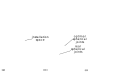
\includegraphics[width=1.0\linewidth]{workspaces.pdf}
	\caption{Workspace of the proposed parallel robot with platform tilt angle of \SI{0}{\degree} (a), \SI{-10}{\degree} (b), \SI{-20}{\degree} (c)}
	\label{fig:workspace}
	\vspace{-5mm}
\end{figure}
Given the final design, further evaluations of \emph{workspace characteristics} are provided, which are out the scope of the dimensional synthesis due to their high computational effort. 
Still, the workspace is important for the application since the reference trajectory does not guarantee a gapless workspace. %, a workspace analysis was performed, using the kinematics model. 
In addition to the kinematic limits themselves, the workspace also suffers from truncation due to inherent collision, installation space and joint angle limits, where the spherical joint's tilt angles are dominant. 
The workspace is calculated specifying a fixed platform tilting angle (by using $\varphi_x$ and $\varphi_y$ from  intrinsic $X$-$Y$-$Z$ Cardan angles). 
Any rotation $\varphi_z$ around the tool axis is allowed (subject to other constraints), as this represents the redundant coordinate. 
Therefore, the computed workspace volumes correspond to the constant-orientation workspace regarding the reduced orientation of the 3T2R task, cf.\,\cite{Merlet2006}.
The platform tilt angle is set to \SI{0}{\degree}, \SI{-10}{\degree} and \SI{-20}{\degree} using $\varphi_y$, visualized in Fig.\ref{fig:workspace}. 
First, leaving aside the mentioned design-related limitations and only assuming a tilt angle limit of \SI{29}{\degree} (considered the best case of a real rod end bearing), the workspace with a total volume between \SI{0.522}{\cubic\metre} ($\varphi_y = \SI{0}{\degree}$) and \SI{0.389}{\cubic\metre} ($\varphi_y = \SI{-20}{\degree}$) can be seen in Fig. \ref{fig:workspace} (volumes colored gray), as this gives an undistorted view of the characteristics of the actual kinematic structure.
Due to the requirements of the weed control process and the derived reference trajectory, a relatively large workspace can be obtained.
%A high volume is the result, due to the requirements of the process and the reference trajectory. 
The workspace decreases especially in the radius and shifts laterally in $x$-direction, with increasing platform orientation. 
In relation to the sketched installation space, which is defined upwards starting at $z=0$, the workspace fills a high proportion of the volume. 
Structures determined in the synthesis are not allowed to exceed this limitation, because this plane represents the ground.
Taking the restrictions of the installed spherical joints into account, the resulting workspace volumes are presented in the figure as well (volumes colored green). 
The remaining volume amounts \SI{0.205}{\cubic\metre} ($\varphi_y = \SI{0}{\degree}$) and \SI{0.125}{\cubic\metre} ($\varphi_y = \SI{-20}{\degree}$). 
% Although there is a loss of volume in the peripheral area in radial direction, this meets the requirements of the process and is therefore suitable for the intended purpose. 
Although there is a loss of volume in the peripheral area (radial direction), this meets the requirements of the weed control process. Therefore the kinematic is suitable for the intended purpose. 

%%% Notizen
% - workspace\\
%     * constant pointing direction\\
%     * additional restriction due to real components: igus u-joints\\
% - 2 plots:\\
%     * unbeschränkter (Bauraum/u-joints) + beschränkt\\
%     * ggf. zusätzlich mit 10/20° Kippwinkel\\
%     * Trajektorie rein?\\
% 	* ggf. Quader rein?\\
% 		* für Bauraum\\
% 		* großer Teil des Arbeitsraum gar nicht für Anwendung und Synthese relevant\\
% - singularities\\
% - compare with standard Hexa (-> synthesis)\\


\section{Conclusion}
As a result of synthesis and design of parallel kinematics for weeding, a novel variant of the well-known \textsc{Hexa} robot is presented. The special characteristic consists in inclined cranks and the configuration with elbows directed inwards, which allows a compact design. The workspace characteristics examined are suitable for the intended weeding application and benefits are also promising for other applications with similar requirements. 
%
% - neue variante des Hexa\\
% - nach innen geneigte Ellenbogenkonfigration\\
% - Leistungsmerkmale (gut), geeignet\\
%
\section*{Acknowledgement}
The project is supported by funds of the Federal Ministry of Food and Agriculture (BMEL) under grant number 2818812B19. 
The synthesis toolchain was funded by the German Research Foundation (DFG) under grant number 341489206.
\textsc{Matlab} code to reproduce the synthesis' results and figures is available at GitHub under free license at \url{github.com/SchapplM/robotics-paper_i4sdg2023}.

% ---- Bibliography ----
% \bibliographystyle{splncs04}
\bibliographystyle{splncs03_unsrt}
\bibliography{references}

\end{document}